% configuração da fonte, pode ser courier ou times

\documentclass[courier]{uninove-ppgi}

% local definitions (utilizado para controlar a posição do número da equação)

\newcommand{\numberequation}[1]{\addtocounter{equation}{#1}\tag{\theequation}}

\begin{document}

% parametros de capa e folha de rosto (é necessário configurar todos)

\Universidade{UNIVERSIDADE NOVE DE JULHO - UNINOVE}
\Programa{PROGRAMA DE PÓS GRADUAÇÃO EM INFORMÁTICA E GESTÃO DO CONHECIMENTO - PPGIGC} 	
\Autor{CHARLES FERREIRA GOBBER}	 
\Titulo{ÚLTIMOS LEVELINGS COM BASE EM FUNÇÕES DE ENERGIA APLICADOS A DETECÇÃO DE OBJETOS}
\Tipoexame{Qualificação}
\Titulacao{Mestre}
\Orientador{Dr. Wonder Alexandre Luz Alves}
\Ano{2017}


% gera a capa

\capa


% gera folha de rosto

\folharosto

		   
% configurações do resumo em portugues

\PalavrasChave{Últimos levelings, Funções de energia, Mumford-Shah, Árvores de componentes, Árvore de formas.}

\begin{resumo}

Bla bla bla

\end{resumo}


% configurações do resumo em inglês

\KeyWords{Ultimate levelings, Energy functions, Mumford-Shah, Component tree, Tree of shapes.}

\begin{abstract}

Bla bla bla

\end{abstract}

% Sumário

\tableofcontents 
\thispagestyle{empty}
		   
% Lista de figuras

\listoffigures
\thispagestyle{empty}

% Lista de algoritmos

\listofalgorithms
\thispagestyle{empty}

% lista de abreviaturas (não colocar espaçamentos adicionais, pois eles contam dentro do environment)

\begin{listaabreviaturas}%
	MM & Morfologia matemática \\
	CC & Componente conexo \\
	EE & Elemento estruturante \\
	MS & Mumford-Shah \\
	\textit{poset} &  Acrônimo para a expressão em inglês \textit{partially ordered set}\\
				   &  (em português: conjunto parcialmente ordenado) \\
	\textit{pixel} &  Acrônimo para a expressão em inglês \textit{picture element}\\
				   &  (em português: elemento da imagem)
\end{listaabreviaturas}

% lista de símbolos (não colocar espaçamentos adicionais, pois eles contam dentro do environment)
% atualmente a lista não suporta multiplas páginas, ou seja ela quebra a lista inteira.

\begin{listasimbolos}%
	\simbolos{Conceitos básicos} {%		
		$ \mathbb{Z} $ & Conjunto dos números inteiros \\						
		$ \mathbb{N} $ & Conjunto dos números naturais \\		
		$ \mathbb{R}^+ $ & Conjunto	dos números reais positivos \\	 		
	}
	\simbolos{Imagens} {%	
		$ f $ & Váriavel que representa uma imagem \\			
		$ \mathcal{D} $ & Conjunto que representa o domínio da imagem \\					
		$ \mathbb{K} $ & Conjunto que representa o contradomínio da imagem \\		
	}
\end{listasimbolos}

% Corpo do documento

\chapter{Exemplo de capítulo}

\begin{resumocapitulo}
As seções e subseções são configuradas de acordo com a norma ABNT adotada pela Uninove (tamanho da fonte, espaçamento...). As numerações de página estão alinhadas a direita no \textit{header}.
\end{resumocapitulo}

\section{Exemplo de seção}

\subsection{Exemplo de subseção}

Alguns comandos matemáticos também estão disponíveis, pode-se criar definições, proposições e provas:

\begin{definicao}{Média aritmética}
Para uma amostra $ X=\{x_1,, x_2, \ldots,x_n\} $ de observações, onde $ n $ é o número de observações, se define a média aritmética da seguinte forma:
\begin{equation}
\mu(X)=\dfrac{1}{n}\sum\limits_{x \in X}x
\end{equation}
\end{definicao}
\begin{proposicao}
Se $ k $ é uma constante então multiplicar a média de uma amostra $ X $ é o mesmo de multiplicar cada elemento de $ X $ por $ k $, isto é, $ k \times \mu(X) = \dfrac{1}{n} \sum\limits_{x \in X}x\times k $.
\end{proposicao}
\begin{prova}
Desenvolve-se a igualdade:
\begin{align*}
k \times \mu(X) &= \dfrac{1}{n} \sum\limits_{x \in X}xk \\
& \Longleftrightarrow  \dfrac{(x_1k,x_2k, \ldots, x_nk)}{n} \\
& \Longleftrightarrow  \dfrac{nk \times (x_1,x_2, \ldots, x_n)}{n} \\
& \Longleftrightarrow   k \times \dfrac{(x_1,x_2, \ldots, x_n)}{n} \\
& \Longleftrightarrow   k \times \mu(X) \numberequation{1}
\end{align*}
\end{prova}
Assim, concluí-se que $ k \times \mu(X) = \dfrac{1}{n} \sum\limits_{x \in X}x\times k $. $ \square $
 
\subsubsection{Exemplo de subsubseção}

Figuras também estão configuradas pela norma ABNT, a legenda é centralizada e a fonte da figura é recuada a esquerda:

\begin{figure}[ht!]

	\begin{center}
	
		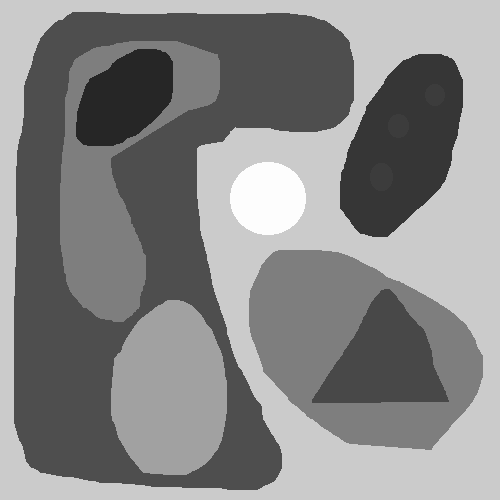
\includegraphics[scale=0.4]{leveling1}
	
	\end{center}
	
	\caption{Uma imagem.}
	
	\fonte{\citeonline{alves:article:2017} (Adaptado pelo autor)}
	
\end{figure}

As citações podem ser feitas de duas formas: {\color{red}$\backslash$citeonline}\{chave da citação\} = \citeonline{seymor:book:1971} e {\color{red}$\backslash$cite}\{chave da citação\} = \cite{seymor:book:1971}. Note que, nas referências bibliográficas o título está em negrito, de acordo com a norma ABNT 6023, para este efeito é necessário incluir a entrada no arquivo bibtex (refs.bib).

Exemplo simples de pseudocódigo utilizando o pacote {\color{red}algorithm2e} configurado para língua portuguesa:

% controla identação
\begin{algorithm}[H]
\SetAlgoLined
\Entrada{$S,\eta, U$} 
\Saida{Número esperado de nós atingidos}
\Inicio{
	$\sigma(S) = 0$ \\
\Para{cada $u \in S$}{
	$\sigma(S)\leftarrow \sigma(S)+\textsc{Backtrack}(u,\eta,W,U)$\\
}
}
\Retorna{$\sigma(S)$}
\label{alg1}
\caption{\textsc{Esperança}}
\end{algorithm}

% Incluindo bibliografia

\bibliography{refs}
		   
\end{document}